\documentclass[conference]{IEEEtran}

\usepackage[utf8]{inputenc}
\usepackage[T1]{fontenc}
\usepackage{amsmath}
\usepackage{amssymb}
\usepackage{graphicx}
\usepackage{booktabs}
\usepackage{listings}
\usepackage{xcolor}
\usepackage{tikz}
\usetikzlibrary{shapes.geometric, arrows.meta, positioning, fit, backgrounds}
\usepackage{url}
\usepackage{cite}
\usepackage{microtype}

% Vertical spacing between top/bottom floats and body text
\setlength{\textfloatsep}{10pt plus 4pt minus 2pt}
\setlength{\floatsep}{8pt plus 2pt minus 2pt}
\setlength{\intextsep}{8pt plus 2pt minus 2pt}

\lstdefinelanguage{pseudo}{
  morekeywords={citeste,scrie,daca,atunci,altfel,sf,cat,timp,executa,
                pentru,repeta,pana,cand,si,sau,nu,not,and,or},
  sensitive=false,
  morecomment=[l]{\#},
  morestring=[b]",
}

\lstset{
  basicstyle=\ttfamily\footnotesize,
  breaklines=true,
  frame=single,
  columns=flexible,
  keywordstyle=\bfseries,
  commentstyle=\itshape\color{gray},
  stringstyle=\color{black},
  framesep=3pt,
  xleftmargin=4pt,
  xrightmargin=4pt,
  aboveskip=6pt,
  belowskip=4pt,
}

\begin{document}

\title{Pseudo++: A Browser-Based Toolchain for\\Romanian Baccalaureate Pseudocode}

\author{
  \IEEEauthorblockN{Bujor Mihai Alexandru}
  \IEEEauthorblockA{
    Faculty of Mathematics and Computer Science\\
    Babe\c{s}-Bolyai University, Cluj-Napoca\\
    bujormihaialexandru@gmail.com
  }
  \and
  \IEEEauthorblockN{Rares Florin Boian}
  \IEEEauthorblockA{
    Faculty of Mathematics and Computer Science\\
    Babe\c{s}-Bolyai University, Cluj-Napoca
  }
}

\maketitle

% ─────────────────────────────────────────────────────────────────────────────
\begin{abstract}
The Romanian national baccalaureate examination in Computer Science requires
candidates to read, write, and reason about programs expressed in a pseudocode
dialect that uses Romanian keywords, Unicode mathematical symbols, and a
box-drawing block structure.  Despite being central to the secondary-school CS
curriculum, this dialect has never had a standard execution environment:
students must trace programs by hand, with no automated way to verify
correctness.

This paper presents \textbf{Pseudo++}, an open-source toolchain that fills
this gap.  The toolchain is built around a single C library compiled to both a
native binary and a WebAssembly module, ensuring identical behaviour in the
command-line interface and the browser-based web editor.  It comprises eight
components: a Tree-sitter grammar formally capturing the dialect's syntax; a
two-pass formatter normalising Unicode and ASCII notation; a tree-walking
interpreter with an explicit execution stack; a step-through debugger with
live variable and condition inspection; a two-pass transpiler generating C,
C++, or Pascal; a loop-equivalence module converting between all four loop
constructs; a browser-based editor built on Monaco and Emscripten that runs
entirely offline; and a CLI for scripting and batch use.

The toolchain is evaluated on 53 official Romanian baccalaureate problems
spanning six examination years (2020--2025), achieving a 100\,\% pass rate.
The transpiler produces compilable, warning-free C for all 32 verified
problems, and all 9 directed loop-equivalence conversions preserve observable
output exactly.  Pseudo++ is the only tool that combines execution, debugging,
transpilation, and static analysis for this dialect in a single browser-based
environment.
\end{abstract}

\begin{IEEEkeywords}
pseudocode interpreter, educational programming tools, WebAssembly,
transpiler, Romanian baccalaureate, Tree-sitter
\end{IEEEkeywords}

% ─────────────────────────────────────────────────────────────────────────────
\section{Introduction}
\label{sec:intro}

The Romanian national baccalaureate examination in Computer Science requires
candidates to read, write, and reason about programs in a pseudocode dialect
established by convention through high-school CS textbooks and examination
papers~\cite{romanian-curriculum}.  The dialect uses Romanian keywords
(\textit{cite\c{s}te}, \textit{scrie}, \textit{dac\u{a}}, \textit{c\^{a}t
timp}, \textit{pentru}, \textit{repet\u{a}}), Unicode mathematical symbols
for assignment and comparison ($\leftarrow$, $\leq$, $\geq$, $\neq$), and
box-drawing characters (\texttt{┌}, \texttt{│}, \texttt{└}, \texttt{■}) for
visual block structure.

Despite being one of the core notations in Romanian secondary CS education,
this dialect has no standard execution environment.  Students must trace
programs by hand.  Manual tracing develops intuition but is error-prone for
longer programs and provides no automated feedback.  The dialect cannot be fed
to any general-purpose language tool: its Unicode symbols and Romanian keywords
are not valid in C, C++, or Pascal.  General pseudocode interpreters designed
for other language curricula do not recognise the Romanian syntax, and the only
existing browser-based tool for Romanian pseudocode (pseudocod.ro) diverges
from the baccalaureate standard in significant ways~\cite{pseudocodro}.

This paper presents \textbf{Pseudo++}, a complete open-source toolchain that
addresses this gap.  Section~\ref{sec:dialect} describes the pseudocode dialect
and its parsing challenges.  Section~\ref{sec:related} surveys related work.
Section~\ref{sec:design} presents the system architecture.
Section~\ref{sec:components} details the eight core components.
Section~\ref{sec:evaluation} reports the evaluation results.

% ─────────────────────────────────────────────────────────────────────────────
\section{The Baccalaureate Pseudocode Dialect}
\label{sec:dialect}

\subsection{Notation and Language Features}

The dialect combines Romanian keywords, Unicode mathematical symbols, and a
visual indentation system based on box-drawing characters.  Listing~\ref{lst:example}
shows a representative fragment from the 2020 baccalaureate training set: the
program reads a natural number \texttt{n} and computes a function of its
digits.

\begin{lstlisting}[language=pseudo, caption={A 2020 baccalaureate training problem in canonical Unicode notation.}, label=lst:example, float=t]
citeste n
p <- 1; m <- 0; k <- 0
cat timp n != 0 executa
    citeste x
    pentru i <- 1, k executa
        x <- [x / 10]
    sf
    daca x != 0 atunci
        c <- x % 10
    altfel
        c <- n % 10
    sf
    m <- c * p + m
    n <- [n / 10]; p <- p*10; k <- k+1
sf
scrie m
\end{lstlisting}

The language supports all four loop constructs (\texttt{cat timp}/while,
\texttt{pentru}/for, \texttt{executa\ldots cat timp}/do-while,
\texttt{repeta\ldots pana cand}/repeat-until), conditional branching
(\texttt{daca\ldots atunci\ldots altfel}), I/O (\texttt{citeste}/\texttt{scrie}),
assignment ($\leftarrow$), the swap operator
(\texttt{x $\leftrightarrow$ y}), floor division (\texttt{[expr]}),
square root ($\sqrt{\phantom{x}}$), modulo, and single-line comments
(\texttt{\#}).  Multi-statement lines separated by semicolons are also
supported.  There are no user-defined functions or arrays:
scalar arithmetic is the full extent of the dialect.

\subsection{Parsing Challenges}

Three properties make the dialect non-trivial to parse.  First, the canonical
form mixes Unicode characters with ASCII text, requiring normalisation before
a standard parser can process it.  Second, block structure is encoded via
box-drawing characters (\texttt{│} as indentation, \texttt{■} as a block
closer), not keywords --- these must be translated to whitespace and the
\texttt{sf} keyword.  Third, the dialect has no official formal grammar: it is
defined implicitly through the corpus of textbooks and past examination papers,
meaning that a grammar formalisation requires a thorough study of all
syntactically valid forms, including edge cases such as multi-statement lines
and optional loop step arguments.

% ─────────────────────────────────────────────────────────────────────────────
\section{Related Work}
\label{sec:related}

\textbf{PSeInt}~\cite{psint} is the closest analogue: a desktop pseudocode
interpreter and debugger for the Spanish-speaking educational community.  It
requires installation, does not recognise Romanian keywords or Unicode
mathematical symbols, and provides no transpiler.  Having been actively
developed for over two decades it has accumulated a large user base across
Latin America, demonstrating the appetite for dialect-specific pseudocode
tooling --- an appetite that no equivalent tool has yet served for Romanian.

\textbf{RAPTOR}~\cite{raptor} and \textbf{Flowgorithm}~\cite{flowgorithm} take
a flowchart-based approach.  Flowgorithm can export to C and C++, making it
the closest existing analogue to Pseudo++'s transpiler, but its input is a
graphical flowchart rather than text, so it cannot process the notation that
appears on Romanian exam papers.

\textbf{Pseudocod.ro}~\cite{pseudocodro} is the only browser-based tool that
targets Romanian pseudocode directly.  Its accepted syntax diverges from the
baccalaureate standard, requiring students to manually adapt programs.  It
provides basic execution only: no debugger, no transpiler, no static analysis,
and no loop-equivalence feature.

Online platforms such as Replit~\cite{replit} and OnlineGDB~\cite{onlinegdb}
require translation to a real language.  Python Tutor~\cite{pythontutor}
provides step-through visualisation but only for mainstream languages.  Its
variable-inspection panel --- a live display of name, value, and type updated
after every statement --- is the closest precedent for Pseudo++'s debugger
view, but it cannot process any form of pseudocode.

Ben-Ari~\cite{benari2001} identifies the conceptual gap between pseudocode and
executable code as a persistent difficulty for learners and advocates for tools
that make the connection explicit and mechanical.  Pseudo++'s transpiler
addresses this gap for the specific case of the Romanian baccalaureate dialect.

Table~\ref{tab:comparison} summarises the feature comparison.
Pseudo++ is the only tool with all six capabilities; none of the surveyed tools
natively executes the Romanian baccalaureate dialect.

\begin{table}[h]
\centering
\small
\setlength{\tabcolsep}{3pt}
\caption{Feature comparison of educational programming tools.  \textit{Trans}:
  transpilation to a compilable language.  \textit{Lint}: static
  analysis / semantic warnings.  \textit{Web}: browser-based, no installation.
  \textit{OSS}: open source.}
\label{tab:comparison}
\begin{tabular}{lcccccc}
\toprule
\textbf{Tool} & \textbf{Exec} & \textbf{Debug} & \textbf{Trans} &
\textbf{Lint} & \textbf{Web} & \textbf{OSS} \\
\midrule
Pseudocod.ro  & \checkmark & $\times$   & $\times$   & $\times$   & \checkmark & $\times$   \\
PSeInt        & \checkmark & \checkmark & $\times$   & $\times$   & $\times$   & \checkmark \\
RAPTOR        & \checkmark & \checkmark & $\times$   & $\times$   & $\times$   & $\times$   \\
Flowgorithm   & \checkmark & \checkmark & \checkmark & $\times$   & $\times$   & $\times$   \\
Replit        & \checkmark & partial    & $\times$   & $\times$   & \checkmark & $\times$   \\
Python Tutor  & \checkmark & \checkmark & $\times$   & $\times$   & \checkmark & \checkmark \\
\textbf{Pseudo++}     & \checkmark & \checkmark & \checkmark & \checkmark & \checkmark & \checkmark \\
\bottomrule
\end{tabular}
\end{table}

% ─────────────────────────────────────────────────────────────────────────────
\section{System Design}
\label{sec:design}

\subsection{Architecture}

The toolchain is structured as four layers of independent C modules
(Fig.~\ref{fig:arch}).  The \emph{utilities layer} (\texttt{environment},
\texttt{string}, \texttt{hashmap}) provides general data structures.  The
\emph{foundation layer} (\texttt{parser}, \texttt{formatter}, \texttt{I/O})
handles source ingestion and abstract I/O.  The \emph{capabilities layer}
(\texttt{runtime}+\texttt{debugger}, \texttt{transpiler}, \texttt{check},
\texttt{equivalence}) implements the four processing modes.  The
\emph{product layer} exposes the capabilities through two builds: a native
CLI binary and a WebAssembly module compiled by Emscripten~\cite{emscripten}.

\begin{figure}[ht]
\centering
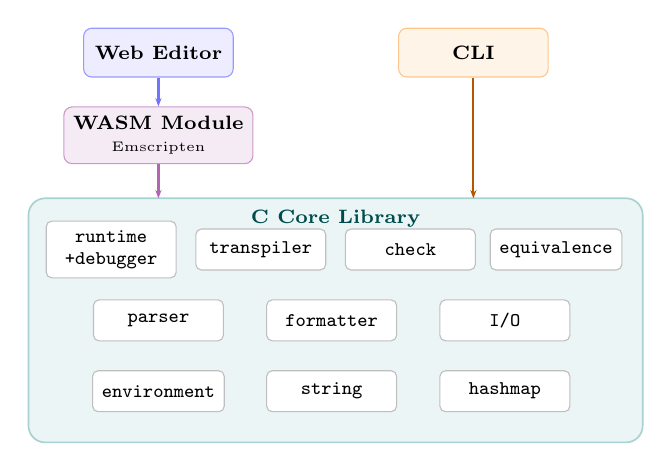
\begin{tikzpicture}[
  box/.style={draw=gray!50, rounded corners=2pt,
              minimum width=1.65cm, minimum height=0.52cm,
              font=\scriptsize\ttfamily, align=center, fill=white},
  prod/.style={draw, rounded corners=3pt,
               font=\scriptsize, align=center,
               minimum width=1.9cm, minimum height=0.62cm},
  arr/.style={-{Stealth[length=3pt]}, thick},
]
\begin{pgfonlayer}{background}
  \fill[teal!8, rounded corners=6pt] (-0.15,-0.35) rectangle (7.65,2.75);
  \draw[teal!35, line width=0.6pt, rounded corners=6pt]
        (-0.15,-0.35) rectangle (7.65,2.75);
\end{pgfonlayer}
\node[font=\scriptsize\bfseries\color{teal!60!black}, anchor=north]
  at (3.75,2.72) {C Core Library};

\node[box] (rt)  at (0.9, 2.1) {runtime\\+debugger};
\node[box] (tr)  at (2.8, 2.1) {transpiler};
\node[box] (chk) at (4.7, 2.1) {check};
\node[box] (eq)  at (6.55, 2.1) {equivalence};

\node[box] (parse) at (1.5, 1.2) {parser};
\node[box] (fmt)   at (3.7, 1.2) {formatter};
\node[box] (io)    at (5.9, 1.2) {I/O};

\node[box] (env) at (1.5, 0.3) {environment};
\node[box] (str) at (3.7, 0.3) {string};
\node[box] (hm)  at (5.9, 0.3) {hashmap};

\node[prod, fill=violet!8, draw=violet!40,
      minimum width=2.4cm]
  (wasm) at (1.5, 3.55) {\textbf{WASM Module}\\{\tiny Emscripten}};

\node[prod, fill=blue!7, draw=blue!40]
  (web) at (1.5, 4.6) {\textbf{Web Editor}};

\node[prod, fill=orange!9, draw=orange!45]
  (cli) at (5.5, 4.6) {\textbf{CLI}};

\draw[arr, blue!55]  (web.south) -- (wasm.north);
\draw[arr, violet!60] (wasm.south) -- (1.5, 2.75);
\draw[arr, orange!70!black] (cli.south) -- (5.5, 2.75);
\end{tikzpicture}
\caption{Pseudo++ module dependency graph.  The C core library is compiled to
  both a native binary (CLI) and a WebAssembly module (Web Editor), sharing
  all execution logic.}
\label{fig:arch}
\end{figure}

\subsection{Single C Core, Two Builds}

A deliberate design decision drives the architecture: the same C source is
compiled twice --- once to a native binary and once to a WebAssembly module.
The I/O layer is the only difference between the two builds.  The CLI uses
\texttt{io\_stdio} (standard \texttt{scanf}/\texttt{printf}); the WASM build
uses \texttt{io\_buffered}, a queue-based mechanism in which JavaScript pushes
input tokens and polls output tokens without blocking the browser's event loop.
All execution, debugging, and transpilation logic is identical.

The WASM bridge exposes the toolchain to JavaScript via
\texttt{EMSCRIPTEN\_KEEPALIVE}-annotated functions:

\begin{lstlisting}[language=C, frame=none]
int   pseudo_init(void);
int   pseudo_load(const char* source);
int   pseudo_step(void);
int   pseudo_run(void);
void  pseudo_push_input(const char* value);
char* pseudo_pop_output(void);
char* pseudo_debug_step(void);
char* pseudo_transpile(const char* src,
                       const char* lang);
\end{lstlisting}

This design guarantees that the browser and terminal interfaces produce
identical output for identical input, with no server component required after
the initial page load.

% ─────────────────────────────────────────────────────────────────────────────
\section{Core Components}
\label{sec:components}

\subsection{Grammar}

The language grammar is specified as a Tree-sitter~\cite{treesitter} grammar.
Tree-sitter generates a GLR parser with incremental re-parsing: edits reuse
unchanged subtrees, giving $O(k \log n)$ amortised complexity for edits of
size $k$~\cite{treesitter-thesis}.  The grammar covers all constructs
described in Section~\ref{sec:dialect}.  When the parser encounters
an unexpected token it inserts \texttt{ERROR}/\texttt{MISSING} sentinel nodes
rather than aborting, so the resulting CST is always complete and serves as a
basis for incremental diagnostics.

The interpreter and transpiler traverse the CST directly via named field
accessors (\texttt{condition}, \texttt{var}, \texttt{start}, \texttt{end},
\texttt{step}), avoiding a separate AST lowering pass.

Expressions follow a standard precedence hierarchy encoded via Tree-sitter's
\texttt{prec.left} operator (Table~\ref{tab:prec}).

\begin{table}[h]
\centering
\small
\caption{Expression precedence levels (lowest to highest).}
\label{tab:prec}
\begin{tabular}{cll}
\toprule
\textbf{Level} & \textbf{Operator(s)} & \textbf{Node type} \\
\midrule
1 & \texttt{SAU} / \texttt{sau} (or)    & \texttt{or\_expr}  \\
2 & \texttt{SI} / \texttt{si} (and)     & \texttt{and\_expr} \\
3 & \texttt{NOT} / \texttt{not}         & \texttt{not\_expr} \\
4 & \texttt{= != < <= > >=}             & \texttt{compare\_expr} \\
5 & \texttt{+ -}                        & \texttt{add\_expr} \\
6 & \texttt{* / \%}                     & \texttt{mul\_expr} \\
7 & \texttt{-(x)}, \texttt{[x]}, $\sqrt{x}$ & \texttt{neg}, \texttt{floor}, \texttt{sqrt} \\
\bottomrule
\end{tabular}
\end{table}

\subsection{Formatter}

The canonical notation uses Unicode characters ($\leq$, $\neq$, $\leftarrow$,
$\blacksquare$, box-drawing bars, Romanian diacritics) that are not accepted
by the parser.  The formatter bridges the two representations in two passes.

\emph{Pass 1 --- Symbol Substitution.}  A static hash map maps Unicode byte
sequences to ASCII equivalents using a greedy maximum-munch strategy
(e.g.\ $\leftarrow$ $\to$ \texttt{<-}, $\leq$ $\to$ \texttt{<=}, the
box-drawing bar U+2502 $\to$ four spaces, $\blacksquare$ $\to$ \texttt{sf}).

\emph{Pass 2 --- Structural Re-indentation.}  All leading whitespace is
stripped and recomputed from scratch based on indent-trigger keywords
(\texttt{atunci}, \texttt{executa}, \texttt{repeta}) and dedent-trigger
tokens (\texttt{sf}, \texttt{altfel}, closing \texttt{pana cand}), producing
a consistently-indented ASCII source.

\subsection{Interpreter}

Runtime values are represented by a heap-allocated tagged union
(\texttt{value\_t}) with three types: \texttt{VALUE\_INT} (\texttt{int64\_t}),
\texttt{VALUE\_FLOAT} (\texttt{double}), and \texttt{VALUE\_STRING}.  Division
always yields a \texttt{double} (matching Romanian textbook convention);
floor division (\texttt{[a/b]}) returns an integer.  Variables are stored in a
flat \texttt{environment\_t}: an open-addressing hash table with linear
probing, FNV-1a hashing~\cite{fnv-hash}, initial capacity 16, and a 70\,\%
load factor.  Variables are implicitly initialised to integer zero.

The interpreter uses an \emph{explicit execution stack} rather than recursion,
serving two purposes: preventing stack overflow for deeply nested programs, and
providing a natural point for the debugger to inspect state.  Each
\texttt{exec\_frame\_t} records the frame type, the corresponding CST node,
and a \texttt{phase} counter encoding progress through the frame's sub-steps.
Frame types are: \texttt{FRAME\_PROGRAM}, \texttt{FRAME\_BLOCK},
\texttt{FRAME\_IF}, \texttt{FRAME\_FOR}, \texttt{FRAME\_WHILE},
\texttt{FRAME\_DO\_WHILE}, \texttt{FRAME\_REPEAT}.  A compile-time dispatch
table maps each type to its step function, making the execution loop a single
indexed function call.  The stack depth is bounded at compile time
(\texttt{MAX\_STACK\_DEPTH = 256}).

Expressions are evaluated by a recursive \texttt{eval\_expr()} function.
Short-circuit evaluation is implemented for the logical connectives:
\texttt{or\_expr} returns 1 immediately if the left operand is truthy;
\texttt{and\_expr} returns 0 immediately if the left operand is falsy.  Error
propagation uses an optional \texttt{value\_error\_t*} out-parameter set on
division-by-zero, type mismatch, or negative square root; any error
transitions the runtime to \texttt{EXEC\_ERROR} and halts execution.  The
\texttt{EXEC\_NEEDS\_INPUT} state suspends execution when a
\texttt{cite\c{s}te} statement encounters an empty input buffer, resuming after
the front end supplies the missing token.

\subsection{Transpiler}

Listing~\ref{lst:transpile} shows the C output produced by the transpiler for
Listing~\ref{lst:example}.

\begin{lstlisting}[language=C, caption={C code generated by the transpiler for the program in Listing~\ref{lst:example}.}, label=lst:transpile, float=t]
#include <stdio.h>
#include <math.h>

int main() {
    int n;
    scanf("%d", &n);
    int p = 1, m = 0, k = 0;
    while (n != 0) {
        int x;
        scanf("%d", &x);
        for (int i = 1; i <= k; i++) {
            x = (int)(x / 10);
        }
        int c;
        if (x != 0) {
            c = x % 10;
        } else {
            c = n % 10;
        }
        m = c * p + m;
        n = (int)(n / 10);
        p = p * 10;
        k = k + 1;
    }
    printf("%d\n", m);
    return 0;
}
\end{lstlisting}

Transpilation proceeds in two passes.  \emph{Pass 1} (\texttt{collect\_vars})
performs a depth-first CST walk and infers each variable's type from its first
assignment: a string literal $\to$ \texttt{string}, a floating-point
literal $\to$ \texttt{double}, otherwise \texttt{int}.  \emph{Pass 2}
(\texttt{gen\_stmt}) emits target code using a \texttt{lang\_ops\_t} record
that encapsulates all language-specific choices (operator syntax, declaration
style, string types), enabling a single pass for all three targets.

Two language-specific concerns are handled explicitly: (1) Pascal's
\texttt{and}/\texttt{or} operators bind more tightly than comparisons, so the
transpiler wraps each operand in parentheses when targeting Pascal; (2) Pascal
string literals use single quotes with doubling for embedded quotes.  Variable
declarations are hoisted inline at the start of each block for C, and into a
global \texttt{var} section for Pascal.

\subsection{Loop Equivalence Module}

The loop equivalence module implements the mutual interconvertibility of all
four loop constructs, grounded in the B\"{o}hm--Jacopini
theorem~\cite{bohm-jacopini} and Dijkstra's structured-programming
principles~\cite{dijkstra1968goto}.  This transformation is an explicit topic
in the Romanian baccalaureate curriculum, and no existing tool provides
automated support for it.

\begin{lstlisting}[language=pseudo, caption={Loop equivalence: a \texttt{pentru} (for) loop (top) converted to a \texttt{cat timp} (while) loop (bottom).}, label=lst:equiv, float=t]
# original
pentru i <- 1, n executa
    scrie i * i
sf

# while equivalent (generated)
i <- 1
cat timp i <= n executa
    scrie i * i
    i <- i + 1
sf
\end{lstlisting}

Given a source string, a 0-indexed target line, and the desired output
construct, the module: parses the source; locates the loop node via DFS;
extracts header fields and body text; constructs the target form; and splices
the new loop back into the source, preserving all surrounding code and
indentation.  Listing~\ref{lst:equiv} shows an example conversion.

Table~\ref{tab:loops} summarises the transformation rule for all twelve directed
pairwise conversions.  The key structural distinction is between \emph{pre-test}
loops (\texttt{for}, \texttt{while}) that may execute zero times and
\emph{post-test} loops (\texttt{do-while}, \texttt{repeat}) that always execute
at least once.  Converting from pre-test to post-test requires a guard
(\textbf{if}~$C$~\textbf{then}) to preserve zero-iteration semantics; the
reverse direction requires duplicating the body before the loop.

\begin{table}[h]
\centering
\scriptsize
\setlength{\tabcolsep}{3pt}
\caption{Loop transformation rules. $B$ = body, $C$ = condition,
  $i/a/b$ = counter/start/end.
  \emph{guard}: wrap with \textbf{if}~$C$~\textbf{then}.
  \emph{dup}: prepend one copy of $B$.}
\label{tab:loops}
\begin{tabular}{l|cccc}
\toprule
From$\backslash$To & \textbf{for} & \textbf{while} & \textbf{do-while} & \textbf{repeat} \\
\midrule
\textbf{for}      & ---
                  & $i\!\leftarrow\!a$; while
                  & $i\!\leftarrow\!a$; guard; do
                  & $i\!\leftarrow\!a$; guard; repeat \\[2pt]
\textbf{while}    & synth$^\dagger$
                  & ---
                  & guard; do
                  & guard; repeat \\[2pt]
\textbf{do-while} & synth$^\dagger$
                  & dup; while $C$
                  & ---
                  & dup; repeat $\neg C$ \\[2pt]
\textbf{repeat}   & synth$^\dagger$
                  & dup; while $\neg C$
                  & dup; do $\neg C$
                  & --- \\
\bottomrule
\multicolumn{5}{l}{$^\dagger$counter variable synthesised from body.}
\end{tabular}
\end{table}

\subsection{Debugger}

After each step, \texttt{runtime\_get\_variables\_json()} serialises the
current variable table to a JSON array of \texttt{\{name, value, type\}}
objects.  When the step involves a conditional or loop guard, the runtime
additionally captures the condition text and its boolean result in a
\texttt{condition\_info\_t} struct.  The WASM bridge combines the variable
table, current line number, execution status, and condition information into a
single JSON response per \texttt{pseudo\_debug\_step()} call.  The web front
end uses this response to highlight the executing source line and update the
variable inspector panel.

\subsection{Static Analysis (\texttt{check} Module)}

The \texttt{check} module traverses the CST after parsing and reports a
structured set of semantic diagnostics without executing the program.
Each diagnostic is assigned a warning code, a source line and column, and a
human-readable message.  Examples include: \texttt{W001} (variable assigned but
never read), \texttt{W002} (variable read before any assignment), and
\texttt{W003} (infinite loop body with no conditional exit).  The \texttt{check}
subcommand in the CLI and the corresponding WASM export (\texttt{pseudo\_check})
return all diagnostics as a JSON array.  This allows the web editor to display
inline gutter markers and the CLI to be used as a linting step in a build
pipeline --- for example, a teacher can batch-check a directory of student
submissions with a single \texttt{pseudo check *.pseudo} invocation.

\subsection{Web Editor}

The web editor is a single-page application built on Monaco
Editor~\cite{monaco} with a custom Monarch~\cite{monarch} tokeniser that
provides syntax highlighting for keywords, operators, strings, numbers, and
comments.  At runtime the JavaScript application loads the compiled WASM module
and communicates with it through the exported C functions, providing Run, Step
Into, Continue, Transpile (with target language selection), Check, and Loop
Equivalence operations.  The editor requires no installation and runs entirely
offline once the page is loaded, making it accessible in school lab
environments where students typically lack administrator rights.

Fig.~\ref{fig:editor} shows the editor with three features active simultaneously.
\emph{Visual Mode} (toggled via the button in the toolbar) renders the
underlying ASCII source as canonical Unicode notation: \texttt{<-}~$\to$~$\leftarrow$,
\texttt{!=}~$\to$~$\neq$, \texttt{sf}~$\to$~$\blacksquare$.
The step-through debugger has advanced to step~9: the currently executing line
is highlighted, the condition panel shows \texttt{n~$\neq$~0}~$\to$~\textsc{true},
and the variable table lists all live bindings with their current values.
The static analyser has marked line~2 with a diagnostic squiggly because
\texttt{x} is assigned but never subsequently read.

\begin{figure*}[t]
\centering
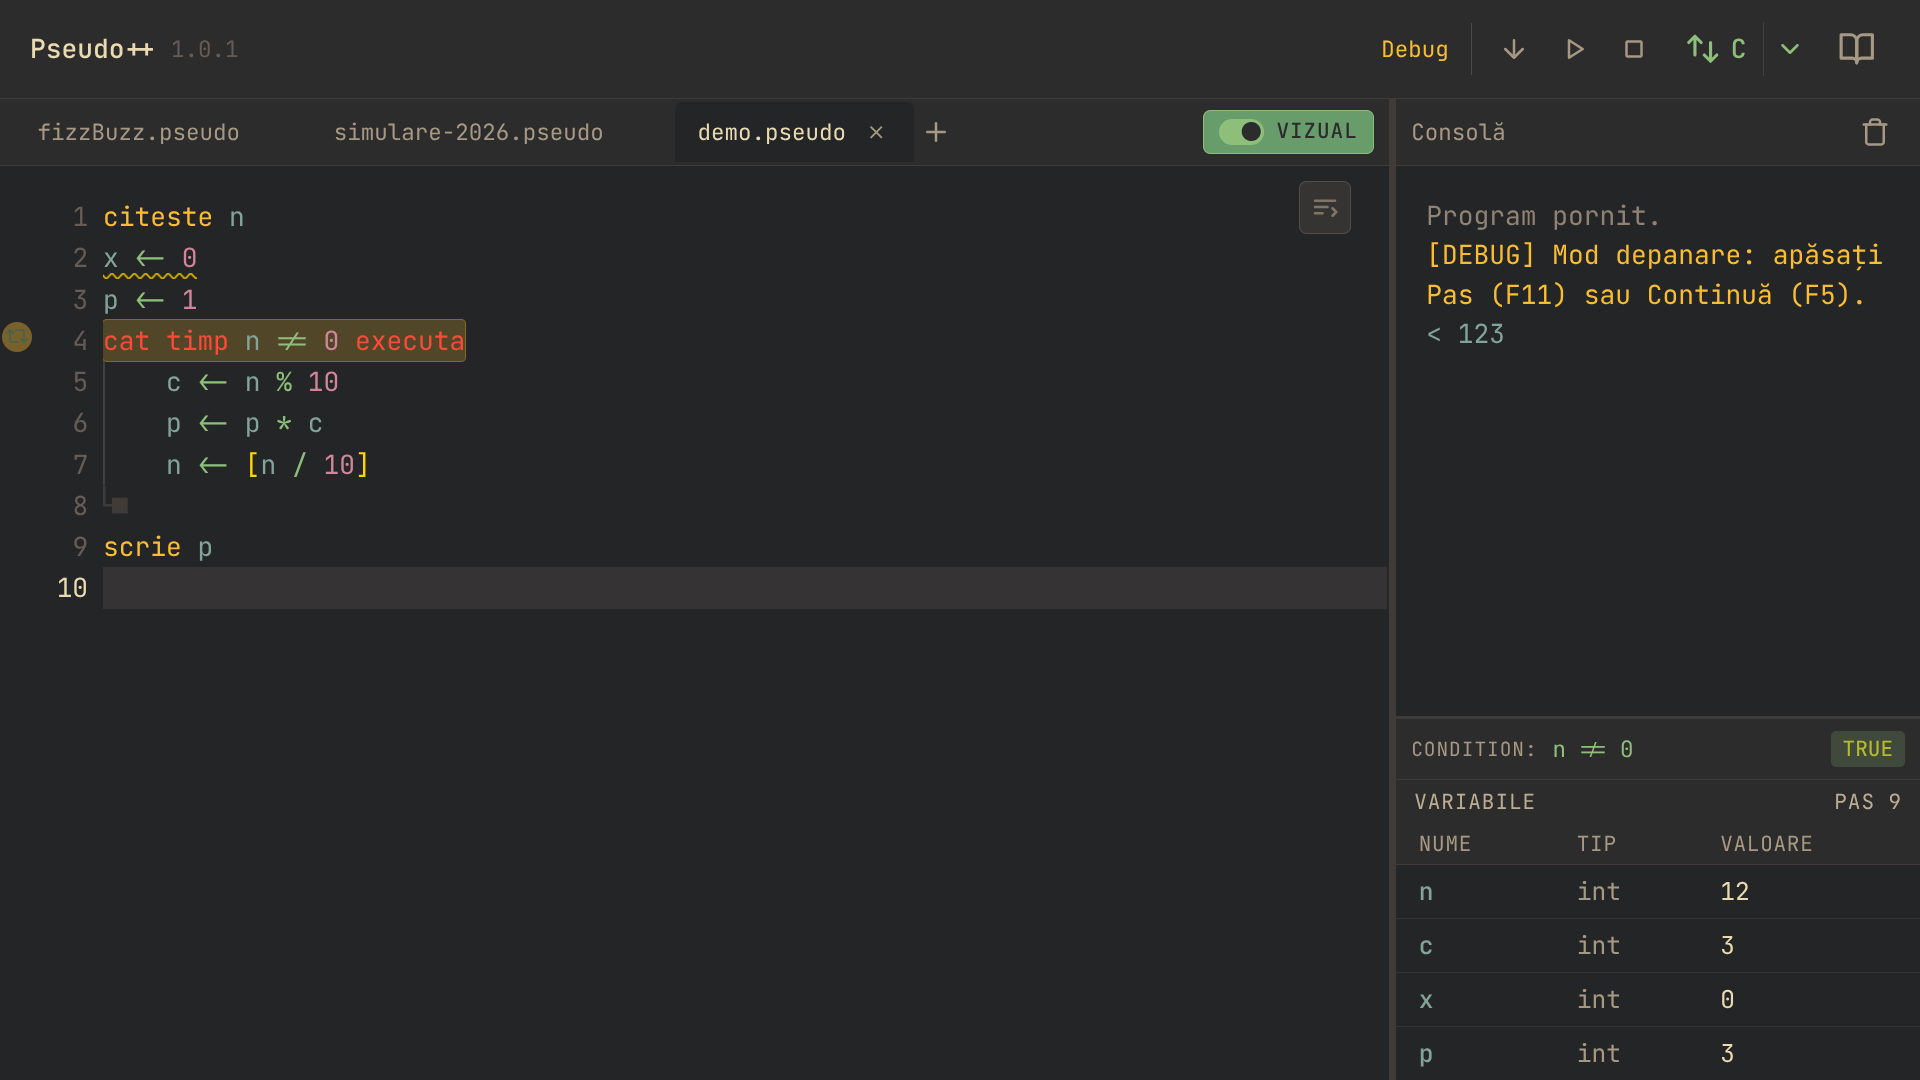
\includegraphics[width=\textwidth]{editor_screenshot.png}
\caption{The Pseudo++ web editor with Visual Mode, step-through debugger, and
  static analysis active simultaneously.
  Line~4 (\texttt{cat timp n~$\neq$~0 executa}) is the current execution
  point; the condition panel confirms \texttt{n~$\neq$~0}~$\to$~\textsc{true}
  and the variable table shows the live state at step~9.
  Line~2 carries a diagnostic squiggly: the static analyser has detected that
  \texttt{x} is assigned but never read (\texttt{W001}).
  Visual Mode is active: assignment arrows, inequality symbols, and the
  block-close square are rendered in Unicode throughout the source pane.}
\label{fig:editor}
\end{figure*}

\subsection{Command-Line Interface}

The \texttt{pseudo} binary exposes the same capabilities as the web editor
through seven subcommands suited to batch processing and scripting:
\texttt{run}, \texttt{format}, \texttt{check}, \texttt{parse},
\texttt{debug}, \texttt{transpile}, and \texttt{equivalence}.
Listing~\ref{lst:cli} shows a representative session: \texttt{check} reports
the unused-variable diagnostic; \texttt{run} executes the program; and
\texttt{transpile} produces C code that GCC compiles to a binary producing
identical output.

\begin{lstlisting}[language=bash, caption={A CLI session: static analysis, execution, and transpilation of the same program.  Diagnostic messages are in Romanian, the target language of the tool.}, label=lst:cli, float=h]
$ pseudo check demo.pseudo
avertisment[W007] la linia 2, coloana 1:
  Variabila 'x' este definita dar niciodata folosita
$ pseudo run demo.pseudo <<< "123"
6
$ pseudo transpile c demo.pseudo | gcc -xc -lm - -o demo
$ ./demo <<< "123"
6
\end{lstlisting}

% ─────────────────────────────────────────────────────────────────────────────
\section{Evaluation}
\label{sec:evaluation}

\subsection{Testing Methodology}

Testing is split across three tiers.  Unit tests (\texttt{make test}) exercise
individual modules in isolation using a minimal \texttt{ASSERT\_STR\_EQ}/\texttt{ASSERT\_INT\_EQ} harness.  Integration tests
invoke the \texttt{pseudo} CLI binary directly with a normalised source file
and compare its standard output byte-for-byte against a reference.  Transpiler
tests extend this pipeline by compiling the generated C with \texttt{gcc -lm}
and running the resulting binary on the same input.

\subsection{Correctness on Baccalaureate Problems}

The integration test dataset consists of 53 pseudocode problems drawn from the
official Romanian baccalaureate training sets published by the Ministry of
Education for examination years 2020--2025 (Table~\ref{tab:dataset}).  The
problems cover all four loop forms, nested conditionals, string and integer
arithmetic, floor-division, modulo, and multi-variable \texttt{cite\c{s}te}
statements.

\begin{table}[h]
\centering
\small
\caption{Baccalaureate integration test dataset.}
\label{tab:dataset}
\begin{tabular}{cr}
\toprule
\textbf{Year} & \textbf{Problems} \\
\midrule
2020 & 20 \\
2021 & 12 \\
2022 &  5 \\
2023 &  5 \\
2024 &  5 \\
2025 &  6 \\
\midrule
\textbf{Total} & \textbf{53} \\
\bottomrule
\end{tabular}
\end{table}

The interpreter correctly produces the expected output for all
\textbf{53 out of 53} problems (\textbf{100\,\%}).  No failures were observed
across any of the six examination years.

\subsection{Transpiler Verification}

Transpiler correctness is verified for the C target on the 32 problems from
the 2020--2021 sets.  All \textbf{32 out of 32} problems (\textbf{100\,\%})
produce compilable C code whose output matches the interpreter reference
exactly.  GCC reported no compilation errors or warnings for any generated
file.  The C++ and Pascal backends share the same emission pass and
\texttt{lang\_ops\_t} abstraction; correctness is established by construction
from the shared code path.

\subsection{Loop Equivalence Semantic Preservation}

The equivalence module is evaluated with 9 directed conversion tests, covering
all ordered pairs among the four loop constructs that change the loop type.
For each test, the module transforms the source loop, the interpreter executes
the result with the original input, and the output is compared against the
untransformed reference.  All \textbf{9 out of 9} transformations
(\textbf{100\,\%}) preserve the program's observable output exactly.

\subsection{Unit Tests}

The formatter module is covered by 39 unit tests verifying symbol
substitution for all entries in the substitution table, greedy maximum-munch
ordering, edge cases (empty input, replacements at boundaries), keyword
normalisation for diacritic variants, and structural re-indentation.
All 39 tests pass.

\subsection{Performance}

Execution time was measured by running each of the 32 baccalaureate problems
100 times in sequence on an AMD Ryzen~5 3600 running Arch Linux with a release
build (\texttt{-O3}).  The mean wall-clock time per problem was
\textbf{2.4\,ms}, dominated by process start-up and the Tree-sitter parse
rather than the interpreter loop itself.  In the web editor the start-up cost
is paid once on module load; subsequent invocations reuse the
already-initialised runtime, confirming sub-100\,ms response times for all
tested problems --- well within the threshold of perceived immediacy.

\subsection{Discussion}

The 100\,\% pass rate across six examination years (2020--2025) and 53
problems validates that the Tree-sitter grammar correctly captures the full
syntax of the dialect as it appears in official Ministry of Education materials,
and that the interpreter faithfully implements the semantics expected in those
materials.  The test set spans the full range of constructs: all four loop
forms, nested conditionals, the floor-division and modulo operators, and
string arithmetic.

The 100\,\% transpiler pass rate (32/32 problems, zero GCC warnings) confirms
that the two-pass variable-type inference heuristic is sufficient in practice:
since the dialect lacks user-defined types, type promotion conflicts that
would require a more sophisticated analysis do not arise.

A notable limitation of the evaluation is that only official baccalaureate
training problems were tested.  These are exclusively short, single-function
programs; edge cases involving deeply nested loops, large inputs, or
adversarial whitespace patterns were not covered by the test suite.  CLI
stress testing and in-browser informal validation confirm the absence of obvious
failures in these scenarios, but a systematic treatment remains future work.

\subsection{Limitations}

Several limitations of the toolchain itself are worth stating explicitly.

\textbf{Scalar variables only.}  The dialect processed by Pseudo++ covers only
scalar types (integers, reals, strings).  Arrays and user-defined functions are
absent from the baccalaureate pseudocode as taught at the secondary level and
are therefore outside the scope of the toolchain; programs requiring indexed
data structures cannot be expressed or executed.

\textbf{Forward-only debugging.}  The debugger supports stepping forward
through execution one statement at a time but does not support stepping
backwards.  Inspecting an earlier program state requires restarting execution
from the beginning.  Snapshot-based reverse debugging~\cite{lewis2003omniscient}
is identified as future work.

\textbf{Heuristic re-indentation.}  The formatter's structural re-indentation
pass is keyword-driven and operates without a full parse.  Pathological source
formatting --- deeply mixed Unicode and ASCII notation or unusual whitespace
structure --- can produce incorrect indentation, causing parse errors for
programs that would otherwise be syntactically valid.

% ─────────────────────────────────────────────────────────────────────────────
\section{Conclusions}
\label{sec:conclusions}

This paper presented Pseudo++, the first open-source toolchain to provide
execution, step-through debugging, transpilation to C/C++/Pascal, static
analysis, and loop-equivalence transformation for the Romanian baccalaureate
pseudocode dialect in a single browser-based, installation-free environment.
The toolchain correctly handles all 53 official baccalaureate problems tested
across six examination years and produces correct, warning-free C code for all
verified transpiler cases.

The single-C-core architecture, compiled to both a native binary and a
WebAssembly module via Emscripten, ensures behavioural parity between the CLI
and the web editor while eliminating any server-side infrastructure requirement.

Directions for future work include: introducing a dialect-agnostic intermediate
representation to support additional Romanian pseudocode dialects (e.g.\ the
Babe\c{s}-Bolyai University admission examination dialect) without duplicating
backend logic; expanding the static analysis module with data-flow diagnostics
such as use-before-assignment and unreachable code detection; adding
snapshot-based step-back debugging; and integrating the WASM module into
existing Romanian educational platforms such as pbinfo.ro as a native
pseudocode execution target.

Pseudo++ is available as open-source software together with the full
integration test suite.

% ─────────────────────────────────────────────────────────────────────────────
\bibliographystyle{IEEEtran}
\bibliography{references}

\end{document}
